\section*{Performance spike analysis}

2018/07/18 - SYNALP - Esteban MARQUER

\subsection{Problem}

During training, a big performance spike appeared periodically. It is
necessary to know why this spike appeared.

The different parts of the spike are:
\begin{itemize}
\item from line 24545 to line 31558 (35\% to 45\% of the corpus): the increase of the BPC;
\item from line 31558 to line 36468 (45\% to 52\% of the corpus): a stable part at a high value;
\item from line 36468 to line 38572 (52\% to 55\% of the corpus): the decrease of the BPC.
\end{itemize}

\begin{longtable}[]{@{}ll@{}}
\hline
Loss of 1 epoch (first epoch) & Zoom on spike\tabularnewline
\hline
\endhead
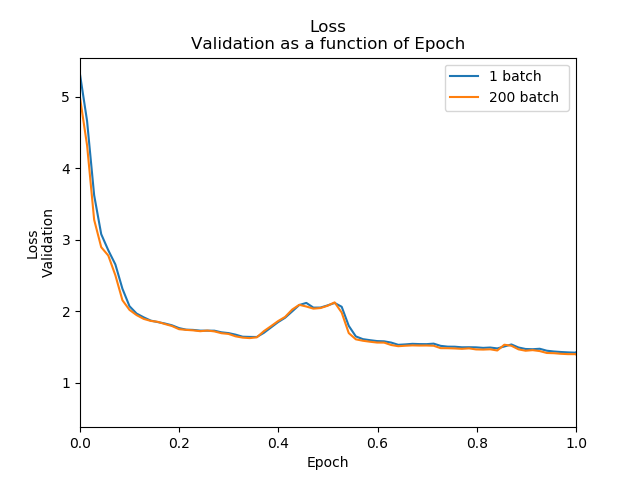
\includegraphics[width=.45\textwidth]{parts/appendix/reports-papud/2018_07_18-Performance_spike_analysis/loss_valid.png} &
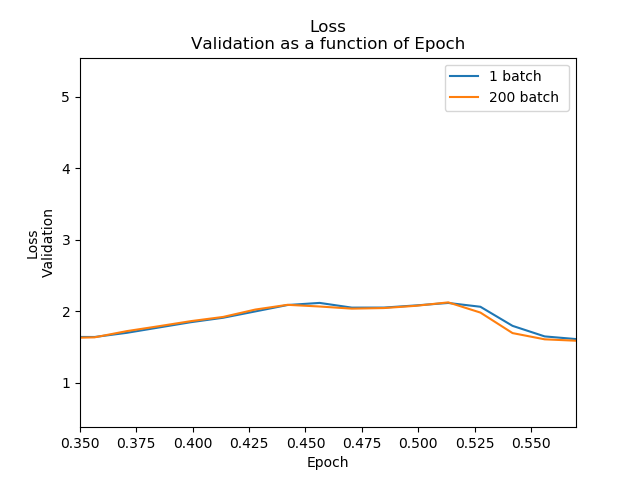
\includegraphics[width=.45\textwidth]{parts/appendix/reports-papud/2018_07_18-Performance_spike_analysis/loss_valid_part.png}\tabularnewline
\hline
\end{longtable}

\subsection{Analysis}

By extracting the parts of the corpus corresponding to the parts of the
spike, and scrolling through them, some recurrent elements appear: -
lines beginning by \lstinline!kern!, more specifically
\lstinline!kern info! and \lstinline!kern debug!; - lines containing a
memory address, like \lstinline!0x91ffffff!, \lstinline!0x0093! and
\lstinline!00000000fed18000!, or an error code like \lstinline!0x0100!,
- lines beginning by \lstinline!daemon!, more specifically
\lstinline!daemon err!;

The most interesting part of the spike is the increase of the BPC, were
the performance deteriorate.

Given the repartition and percentages (see the next two sub-sections),
the most likely causes for the spikes are:
\begin{itemize}
\item the memory address and
hexadecimal codes;
\item the kernel messages (very repetitive, and
containing memory address and hexadecimal codes).
\end{itemize}

\paragraph{Examples of Kernel
messages}

\textbf{Ces données ont été modifiées pour des raisons de confidentialité.}
\begin{lstlisting}
kern info kernel ABCD: FHJLN (abcd_id[0x00] fhjln_id[0x00] enabled)
kern info kernel ABCD: FHJLN (abcd_id[0x02] fhjln_id[0x02] enabled)
kern info kernel ABCD: FHJLN (abcd_id[0x04] fhjln_id[0x04] enabled)
kern info kernel ABCD: FHJLN (abcd_id[0x06] fhjln_id[0x06] enabled)
kern info kernel ABCD: FHJLN (abcd_id[0x08] fhjln_id[0x08] enabled)
\end{lstlisting}

\subsubsection{Repartition of match in the
corpus}

The ``localisation bars'' (vertical blue lines) delimit to the different
parts of the spike.

\begin{longtable}[]{@{}lll@{}}
\hline
Type of element & With localisation bars & With
subcategories\tabularnewline
\hline
\endhead
Memory addresses & 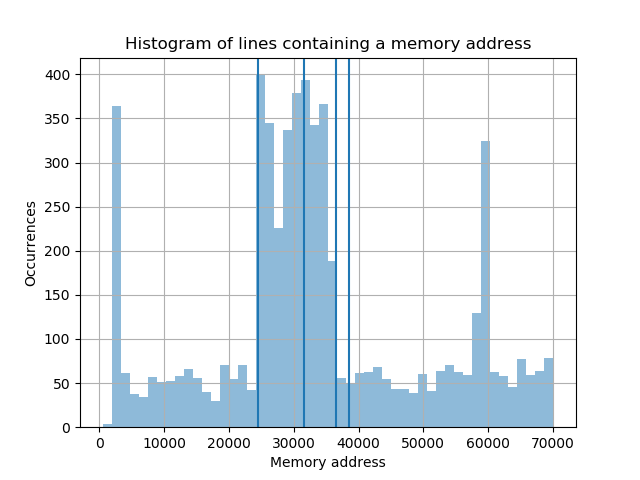
\includegraphics[width=.25\textwidth]{parts/appendix/reports-papud/2018_07_18-Performance_spike_analysis/memory_.png} &
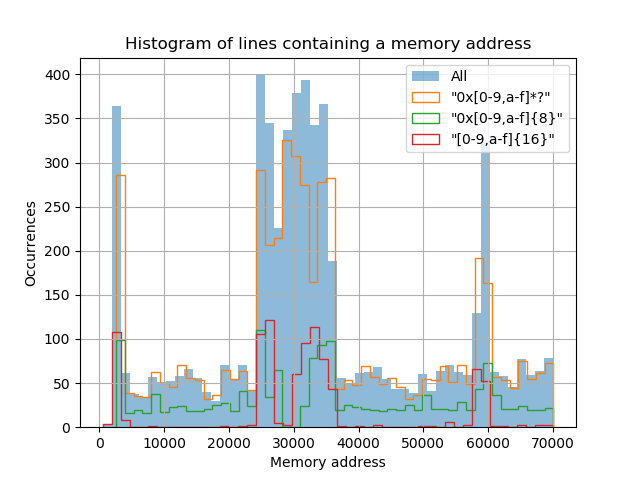
\includegraphics[width=.25\textwidth]{parts/appendix/reports-papud/2018_07_18-Performance_spike_analysis/memory.png}\tabularnewline
Kernel process & 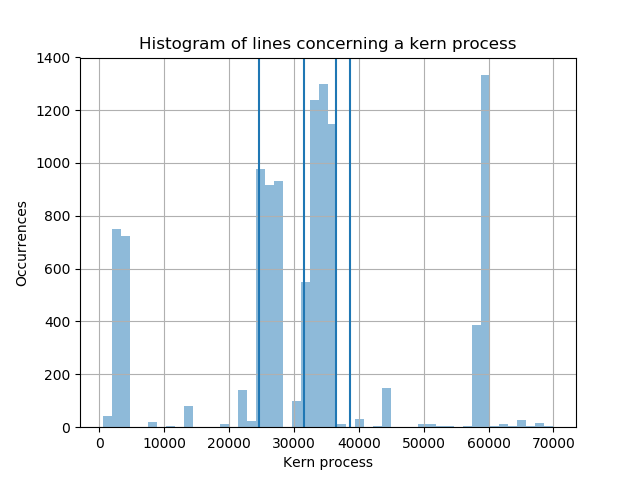
\includegraphics[width=.25\textwidth]{parts/appendix/reports-papud/2018_07_18-Performance_spike_analysis/kern_.png} &
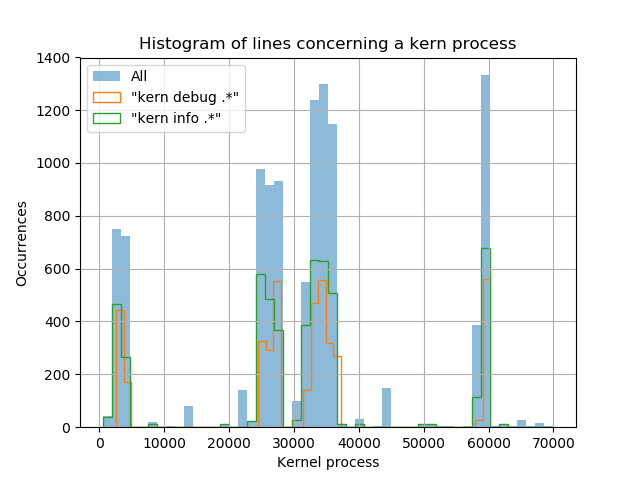
\includegraphics[width=.25\textwidth]{parts/appendix/reports-papud/2018_07_18-Performance_spike_analysis/kern.png}\tabularnewline
Daemon process & 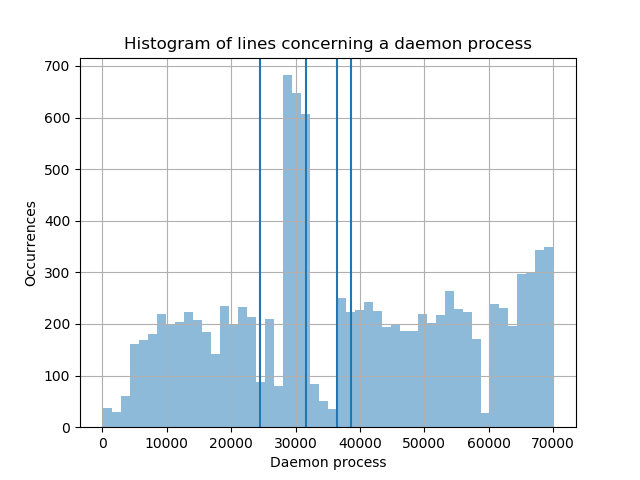
\includegraphics[width=.25\textwidth]{parts/appendix/reports-papud/2018_07_18-Performance_spike_analysis/daemon_.png} &
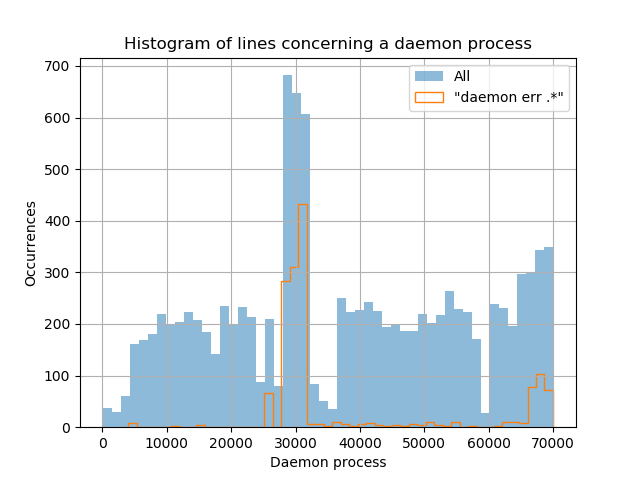
\includegraphics[width=.25\textwidth]{parts/appendix/reports-papud/2018_07_18-Performance_spike_analysis/daemon.png}\tabularnewline
All types & & 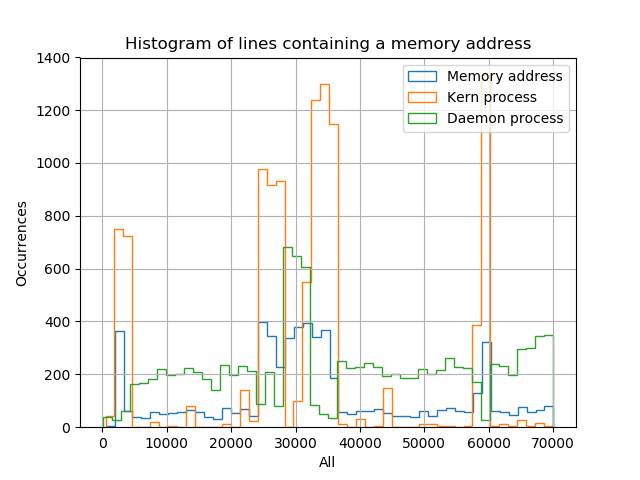
\includegraphics[width=.25\textwidth]{parts/appendix/reports-papud/2018_07_18-Performance_spike_analysis/all.png}\tabularnewline
\hline
\end{longtable}

\subsubsection{Percentages of match in each part of the
corpus}

Percentages of match are percentages on the total line number of the
part of the corpus analysed.

\begin{lstlisting}
--- spike up slope (lines 24545 to 31558, 35% to 45%) ---
Total lines:  7013
Matching "kern .*": 2888 (41%)
Matching "kern info .*": 1458 (20%)
Matching "kern debug .*": 1172 (16%)
Matching "daemon .*": 2048 (29%)
Matching "daemon err .*": 935 (13%)
Matching any memory pattern: 1728 (24%)
Matching "0x[0-9,a-f]{8}": : 196 (2%)
Matching "[0-9,a-f]{16}": : 250 (3%)
Matching "0x[0-9,a-f]*?": : 1478 (21%)

--- spike flat (lines 31558 to 36468, 45% to 52%) ---
Total lines:  4910
Matching "kern .*": 4218 (85%)
Matching "kern info .*": 2154 (43%)
Matching "kern debug .*": 1760 (35%)
Matching "daemon .*": 346 (7%)
Matching "daemon err .*": 174 (3%)
Matching any memory pattern: 1149 (23%)
Matching "0x[0-9,a-f]{8}": : 294 (5%)
Matching "[0-9,a-f]{16}": : 296 (6%)
Matching "0x[0-9,a-f]*?": : 853 (17%)

--- spike down slope (lines 36468 to 38572, 52% to 55%) ---
Total lines:  2104
Matching "kern .*": 27 (1%)
Matching "kern info .*": 15 (0%)
Matching "kern debug .*": 0 (0%)
Matching "daemon .*": 383 (18%)
Matching "daemon err .*": 15 (0%)
Matching any memory pattern: 90 (4%)
Matching "0x[0-9,a-f]{8}": : 34 (1%)
Matching "[0-9,a-f]{16}": : 5 (0%)
Matching "0x[0-9,a-f]*?": : 85 (4%)

--- whole spike (lines 24545 to 38572, 35% to 55%) ---
Total lines:  14027
Matching "kern .*": 7133 (50%)
Matching "kern info .*": 3627 (25%)
Matching "kern debug .*": 2932 (20%)
Matching "daemon .*": 2777 (19%)
Matching "daemon err .*": 1124 (8%)
Matching any memory pattern: 2967 (21%)
Matching "0x[0-9,a-f]{8}": : 524 (3%)
Matching "[0-9,a-f]{16}": : 551 (3%)
Matching "0x[0-9,a-f]*?": : 2416 (17%)

--- full corpus ---
Total lines:  70131
Matching "kern .*": 10972 (15%)
Matching "kern info .*": 5298 (7%)
Matching "kern debug .*": 4134 (5%)
Matching "daemon .*": 10828 (15%)
Matching "daemon err .*": 1504 (2%)
Matching any memory pattern: 5859 (8%)
Matching "0x[0-9,a-f]{8}": : 1586 (2%)
Matching "[0-9,a-f]{16}": : 893 (1%)
Matching "0x[0-9,a-f]*?": : 4987 (7%)

Matching "kern .*" outside of spike: 3839 (5%)
\end{lstlisting}

\subsection{Conclusion(s)}

There are two possible conclusions:
\begin{itemize}
\item the kernel messages are the cause of the spike;
\item or the memory addresses and hexadecimal codes are the cause of the spike.
\end{itemize}

\subsubsection{Kernel messages}

If the kernel messages are the cause of the spike, the most likely
explanation is that this part of the corpus represent a crash of the
server or a major error. In that case, we must remove that part of the
corpus from the training set, as it is not the ``normal'' evolution of
the log.

\subsubsection{Memory addresses and hexadecimal codes}

If the memory addresses and hexadecimal codes are the cause of the
spike, it should be because a succession of number is a very specific
thing to learn. In that case, either we let the model learn the brute
codes, or we replace every code by a ``<hex>'' character to ease the learning
process. It is also possible to replace the different kind of code by a
different character.

\subsection{Improvements and next steps}

To check whether the memory addresses and hexadecimal codes, or the
kernel messages are the cause of the spike, trying to train the model
while replacing every code by a ``<hex>'' character. If there is no
improvement, then the codes are not the cause of the performance spike.
